\lecture{5}{January 18, 2017}{Neha Agarwal, Rohit Agarwal} \\
\section{Introduction}
In the previous lesson we have studied simulated annealing that is a technique to find the global optimum of a given function but we did not study the algorithm implemented in a distributed way, which we will do in this lesson. In addition to this, we will also look at Game theory and its applications.
\\ \\
\section{Simulated Annealing}
Let's assume that we have set $N $ of agents, each agent can choose an action say i choose $a_i \in A_i $. The current state of the system is identified by all the actions chosen by all the agents $S(a_1,a_2,a_3,.....a_N)$, is the state of the system. Let's assume the agents are at the nodes of a system. For simulated annealing  we need to be able to able to consider possible neighbour state of the current state to say if they are better or not in terms of energy and to evaluate the energy for a state. \\ \hfill \break
  Then we change our state $a_1 \longrightarrow a_1'$, we see if the new energy is larger or smaller than the current energy.
  The problem to change the state is easy  to implement in a distributed way as it is enough that one agent by itself decide to change it's action.\\
  If agent 1 change from $a_1 \longrightarrow a_1'$
then automatically we have changed the state. What is more complicated is if agent i change from $a_1 \longrightarrow a_1'$ then the state changes but it is difficult to know how the energy changes.\\ \hfill \break 
As this is a generic function of all the actions can the agent by itself evaluate this function ? \\
If the agent has the function then it can evaluate but if i changes action to $a_i'$     the agent does not know the function the situation is more complex. 
The agent i can change its action but it must be able to evaluate the energy.\\

The energy goes from $E(a_1,a_2,...,a_N) \longrightarrow E(a_1',...,a_N)$ but is the agent 1 able to compute this $\Delta$ of energy. There are some trivial cases where it is possible :-  \\ \hfill \break 
1. YES, if $a_i$ know $E(..,..,..) a_{-i}$, the whole function. where $a_{-i} = (a_1 , a_2 , ... a_N)$.\\ 
This function depends on how many nodes are there, the number of connections and also the state of other agents. This is like solving the global optimization problem if we know the whole function.\\ \hfill \break
2. YES, $E(a_1,...,a_N) = \sum_{i=1}^{N} E_i(a_1)$, completely separable. \\ The function is a sum of only the local energy function that depends on its actions and can implement in a very distributed way the algorithm. Even if it doesn't know all the energy functions as long as it knows its own energy function it can evaluate the $\Delta$ energy because when there is a change in the energy, \\ 
\begin{center}
$\Delta E = E(a_1',a_2...,a_N) - E(a_1,a_2,...,a_N) = E_1(a_1') - E_1(a_1)$
\end{center}\\
even if it doesn't know how many nodes there are what are their energy, it evaluates $\Delta E$ and then decide. \\
The  cases that are distributed are where the energy function can be decomposed and is only a function of energy of actions on cliques. \\
\begin{center}
$E(a_1,a_2,...,a_N)$ = \sum_{c \, \in \,all \, the\, clique\, of \,order \, \leq \, K } V(c)  \\ \\
\end{center}
clique of order 1 are single nodes.\\
If the node can express its energy as the sum of something that depends only on the values of a single node then its done.\\ clique of order 2 are links.\\
If the node can express its function as the sum of energy related to the links then it can still solve in a distributed way the algorithm. The same is for nodes of order 3.\\ \\
If you consider more number of nodes you consider the clique as a single entity that takes decision together. When we have clique of order 1 that decide to change its state then we have a single node that want to change state. Generally when we move to clique of order 2 the link decides. When the link changes its state the two nodes also change their state and they decide what to do. If we go up to clique of size 3 (triangle) the three nodes need to communicate amongst themselves. So the more we increase the order of the clique more communication is required. 
We study clique of order 2 now which can be though of as network links.
\\
\section{Case Study}
 Access points on the same channel whose transmission range is large could overlap and create interference or noise.To avoid interference we generally decide apriori channel and access point to use. If we want the system to dynamically reconfigure it. We want to minimize the power that each access point receive on the same channel. $AP_s = {1,2,...N}$. \\ \\
 \begin{figure} [ht!]
 \centering
 \frame{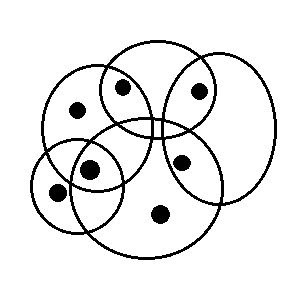
\includegraphics{images/Fig1}}
 \caption{Overlapping transmission of access points }
 \end{figure}
 \hfill \break 
  Assuming all the nodes have the same transmission power .\\  
 \begin{equation}
\begin{aligned}
& \underset{c_1, c_2,..,c_N \, \in \zeta}{\text{minimize}}
\, \, \, \sum_{i=1}^{N} I_i 
& &  =\sum_{i=1}^{N} \sum_{j=1} P_j h_{ji}\, \mathds{1} \,(c_i \,= \,c_j) 
\end{aligned}
\end{equation}
\\
where $P_j$  is power by node j, $h_{ji} $ is fraction of power transmitted by j that arrives to i, $\mathds{1}$ is 1 when $(c_i = c_j)$ and 0 otherwise, $\zeta$ is set of channels available.\\ \\

Every node can solve this independently if every access point knows all the elements for all the access point but it requires a lot of communication.  
Until all the nodes know all the other nodes we not in the first case.\\
For the second case our Interference can be written as sum of local function of energy of the node. 
The eqn (1) gives us this but the function not only depends on that particular node but also the other nodes near it so we are not in the second case.\\
Now we want to see if we are in a condition where the function can be expressed as sum of actions of the links. We see it is a function of links. 
\\ \\
\begin{equation}
\begin{aligned}
& = \sum _{i,j} (P_j h_{ij} \mathds{1} (c_i = c_j ) + P_i h_{ij} \mathds{1} (c_j = c_i))\\ 
\end{aligned}
\end{equation}
Given i for which value of j is this quantity different than zero?\\
Zero only for my neighbours in the interference graph. for the others that are too far $h_{ji} = 0$. \\ \\
\begin{equation}
\begin{aligned}
& = \sum_{e} \mathds{1} (c_i = c_j) (P_j h_{ji} + P_i h_{ij}) \\ 
 \end{aligned}
\end{equation}
\\
Assuming as ever access point transmit at the same power $P_i = P_j $\, ,\,  $h_{ij}=h_{ji}$ we get,\\ 

\begin{equation}
\begin{aligned}
& = 2P \sum_{e} \mathds{1} (c_i = c_j) h_{ji}\\
&  = \sum_{} V_e (c_i = c_j)\\ 
 \end{aligned}
\end{equation}
where  e=(i,j) $\in$ interference graph.\\ \\
If a node i changes its channel it should apriori compute all the interference with it, but with this it need to compute only the neighbours. 
\begin{equation}
\begin{aligned}
& $c_i \longrightarrow c_i' $\\
& \Delta = E(c_i', c_{-i}) - E(c_i', c_{-i})\\  \\
& \Delta = \sum_{j\in N(i)} 2P \mathds{1} (c_j = c_i') h_{ij} - \sum_{j\in N(i)} 2P \mathds{1} (c_j = c_i) h_{ij} \\
 \end{aligned}
\end{equation} 
\\
Node i should be able to  decide independently of going from $c_i \longrightarrow c_i'$ for this node i requires to know \\
$(c_j= c_i) h_{ij}$ which is the power that it hear from the nodes that it hear, the current global interference that it is hearing. \\
If $(c_j \neq c_i )$ then it doesn't listen to that access point and if $(c_j = c_i )$ then it hear $P h_{ij}$ which requires to measure how much power the other access point it can hear  are transmitting on his channel. If they are in other channels it doesn't care.\\ \\
For computing this information required at node i is :-\\
- Inference power on channel $c_i$\\
- Inference power on channel $c_i'$\\
 Then the node doesn't need to ask for information to the other access point. \\ \\
 In Greedy algorithm we see if there is more interference. If no then we stay but if more then we go back .\\ \\ 
 But in simulated annealing we pick a possible different state and then we decide to accept or not. In order to change channel from $c_i $ to $c_i'$ we hear for a while $c_i'$ and then decide, we cannot change every second the channel as every user that are connected to a channel has to even change the channel. \\ \\
If $\Delta$ $E < 0$ then we go to $c_i'$ \\
If $\Delta$ $E > 0$ then we go to $c_i'$ with probability $e^{\frac{\Delta E}{T}}$\\ \\
This can be used when people want to hear something and have to select on which base station to hear.\\ \\ 
If we decrease the temperature where temperature is, 
\begin{equation}
\begin{aligned}
&  T(k) = \frac{T_0}{ln(1+k)}\\
\end{aligned}
\end{equation}
starting from high enough temperature we can optimize the problem and guarantee to converge. We don't require synchronicity so each node can decide independently to change its channel or not. \\
\\ \\
Consider this situation of channel with access point a,b \\ 
\begin{figure} [ht!]
\centering
\includegraphics{images/Fig}
\end{figure}\\
 we have interference but no one want to change as b moving to a would have interference  from other access point that is closer so it doesn't 
 but there is an optimal configuration. 
 If we are greedy we are stuck 
 but with simulated annealing we are sure to converge. 
\begin{figure} [ht!]
\centering
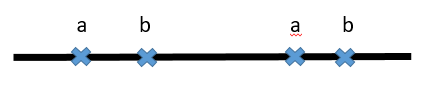
\includegraphics{images/fig}
\end{figure} 

\section{Game Theory}
\textbf{Game theory} is "the study of mathematical models of conflict and cooperation between intelligent rational decision-makers." Originally addressing zero-sum games, where a player's loss is the opponent's gain, now used in many varying fields like economics, computer science, biology, military et. cetra. Before we dive in this chapter, let us get familiarized with some terms and their definitions.

\subsection{Formal Definitions and Terminology}
\begin{enumerate}
    \item Game: A game consists of N-players ($N\geq2)$ where each player $i$ has a set of strategies $S_i$ (mixed or pure) to choose from and an associated pay-off function $P_i$ which maps all element $s \in S_i$ to some real number $r$ in $\mathbb{R}$. 
    \item Pure Strategy: A strategy which provides a complete definition of how a player will play a game. Formally, if player $i$ and player $j$ plays optimally then each of these players could predict the next move of one another.
    \item Mixed Strategy: When a player $i$ chooses a pure strategy randomly from their strategy set $S_i$ then it's called as Mixed strategy. A mixed strategy set $M_i$ has one to one mapping with pure strategy set $S_i$.
    \item Preferential relation $\prec$: We say $P_i(s_k)$ $\prec$ $P_i(s_l)$ when outcome of strategy $s_k$ is worse than strategy $s_l$. Here, $s_k$ and $s_l$ $\in$ $S_i$.
    \item Payoff function $P_i$: This function adds some incentives to each strategy of the user.
\end{enumerate}

\subsection{Game Tree}
A game tree is an extensive form of the real game which explores all the possible outcomes of the game. 
\begin{figure}[h!]
\centering
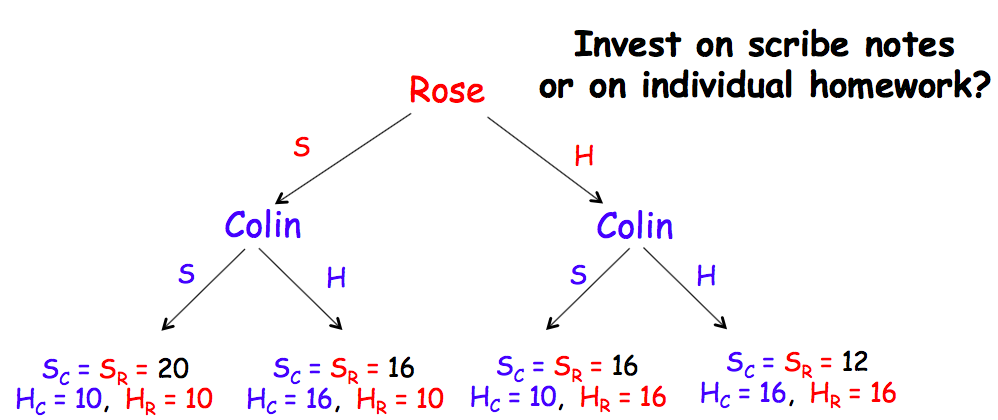
\includegraphics[scale=.35]{images/GameTree}
\caption{Student's Game Tree}
\label{figure1}
\end{figure}

Figure~\ref{figure1} displays a game tree where two students Rose and Colin have to make a decision on investing time on either scribe notes or doing homework with an incentive to maximize their average marks. Here both the players have the same strategy set \{$S$,$H$\}. \\\\We have four possible outcomes:\\
\begin{itemize}
    \item \textit{Case 1}: Rose \textbf{S}, Colin \textbf{S}: If both Rose and Colin invest time on the scribe notes. They receive an average marks of 15 each.
    \item \textit{Case 2}: Rose \textbf{S}, Colin \textbf{H}: If Rose spends time on scribe notes and Colin spends time on homework then they receive average marks of 13 and 16 respectively.
    \item \textit{Case 3}: Rose \textbf{H}, Colin \textbf{S}: If Rose spends time on homework and Colin spends time on scribe notes then they receive average marks of 16 and 13 respectively.
    \item \textit{Case 4}: Rose \textbf{H}, Colin \textbf{H}: If both Rose and Colin invest time on the homework. They receive an average marks of 14 each.
\end{itemize}If both Rose and Colin decides to play optimally at each move i.e they both want to increase their individual average marks then for Rose $P_{rose}(S) \prec P_{rose}(H)$. This is because Rose knows that in the next step Colin will choose homework (\textit{optimal move}) and drive the game to Case $2$ where the average marks of Rose would be 13. However, choosing $H$ would for sure produce an average greater than $13$. So, at the next step Colin chooses homework and they both get an average of $14$.\\\\
Please note here, Case $1$ is better than the current outcome which is Case $3$, with an average of $15$ rather than $14$.  
\subsection{Matrix Game / Normal-form Game}
A Normal-form game or sometimes called as Matrix game is another way of representing a game. As the name suggests, it uses a $N$-dimensional matrix to represent the state space of the game. This representation is very useful to find equilibrium states and dominated strategies which we will see in details later.

\begin{figure}[h!]
\centering
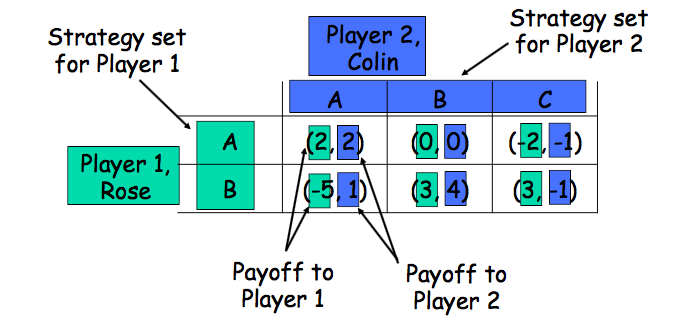
\includegraphics[scale=.35]{images/Normal-form}
\caption{Normal-form example.}
\label{figure2}
\end{figure}

Figure~\ref{figure2} here is a Normal-form example. For player $1$ the strategy set consists of \{A,B\} and for player-$2$ the strategy set consists of \{A,B,C\}. Each cell $C_{i,j}$ in the matrix corresponds to the case when player-$1$ chooses strategy $i$ and player-$2$ chooses strategy $j$. The value of the cell $C_{i,j}$ corresponds to the payoff of each of the players, which is denoted by a tuple $T$ ($t_1$,$t_2$). For example, value of cell $C_{B,C}$ which is the tuple $(3,-1)$, corresponds to the case where player-$1$ would gain $3$ and  player-$2$ would lose 1.\\\\
\begin{figure}[h!]
\centering
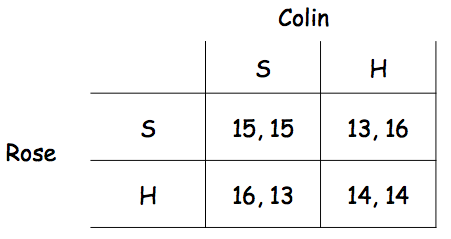
\includegraphics[scale=.35]{images/Normal-form-student}
\caption{Normal-form of the Student's Game Tree}
\label{figure3}
\end{figure}
Figure~\ref{figure3} is an example of the normal-form of our student's game tree in Figure~\ref{figure1}
\subsection{Two Person Zero Sum Games}
A \textbf{zero sum game} is a mathematical representation of a situation in which each participant's gain or loss of utility is exactly balanced by the losses or gains of the utility of the other participants. The corresponding game matrix entry represents payoff gain for only one player. This gain can be any positive or non positive number or 0. A negative gain for a player will be a positive gain for another. For example:-

\begin{figure}[h!]
\centering
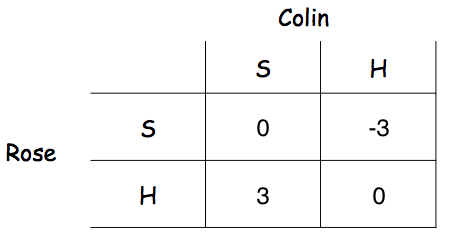
\includegraphics[scale=.35]{images/Normal-form-single-entry-student}
\caption{Single Entry Normal-form of Figure~\ref{figure3}}
\label{figure4}
\end{figure}

\subsection{Dominance}
Dominance is defined over two strategies. Let $S_1$ and $S_2$ be two strategies then:-
\begin{enumerate}
    \item $S_1$ \textit{strictly dominates} $S_2$: If every possible outcome when $S_1$ is chosen is strictly better than corresponding outcome in $S_2$.
    \item $S_1$ \textit{weakly dominates} $S_2$: If every possible outcome when $S_1$ is chosen is at least as good as corresponding outcome in $S_2$, and one is strictly better.
\end{enumerate}
\textbf{Dominance Principle}: This principle states that a rational player will never play a strategy that is dominated by some other strategy.\\\\
\textbf{High order Dominated Principle}: This principle states that we can iteratively remove dominated strategies. In any case, if by iterated elimination of dominated strategies there is only one strategy left for each player, the game is called a dominance-solvable game.\\\\
Let us see an example:-\\
\begin{figure}[h!]
\centering
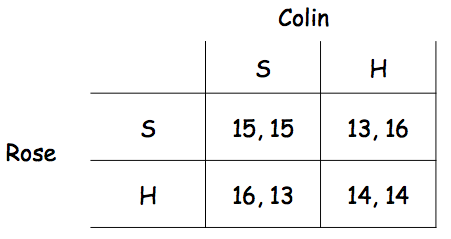
\includegraphics[scale=.35]{images/Normal-form-student}
\caption{Initial matrix}
\label{figure5}
\end{figure}\\
We are given an initial matrix of the game which is represented by Figure~\ref{figure5}. Let Rose be the first person to move.\\
\textbf{Iteration 1}: Rose can either choose strategy $S$ or strategy $H$. Let's look at both the cases:-\\
\begin{itemize}
    \item If rose chooses $S$: Colin can choose either $S$ or $H$. If Colin chooses $S$ then the net gain for Rose is $0$. However, if Colin decides to choose $H$ then Rose has a loss of 3.
    \item If rose chooses $H$: Colin can choose either $S$ or $H$. If Colin chooses $S$ then the net gain for Rose is $3$ and if Colin chooses $H$ then Rose has a loss of 0.
\end{itemize}
So, we see that if rose chooses $S$ she can incurs the gain of $R_1$ = $[0, -3]$ and if she choose $H$ she incurs the gain of $R_2$ = $[3, 0]$. We see that each $i^{th}$ element of $R_2$ is greater than the corresponding $i^{th}$ element of $R_1$. Therefore, $H$ dominate $S$. Our initial matrix now transforms to Figure~\ref{figure6}.
\begin{figure}[h!]
\centering
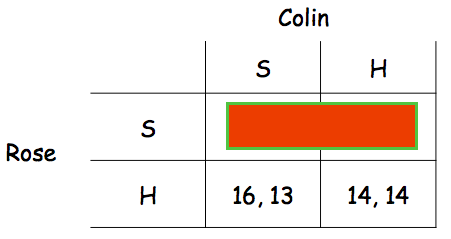
\includegraphics[scale=.35]{images/step1}
\caption{Iteration 1}
\label{figure6}
\end{figure}\\
\textbf{Iteration 2}: It is now Colin's turn and Colin can choose either $S$ or $H$.
We can see here that choosing $H$ over $S$ is more preferable for Colin because he incurs a 0 loss in that case. So, $H$ dominates $S$. Our matrix transforms to Figure~\ref{figure7}.
\begin{figure}[h!]
\centering
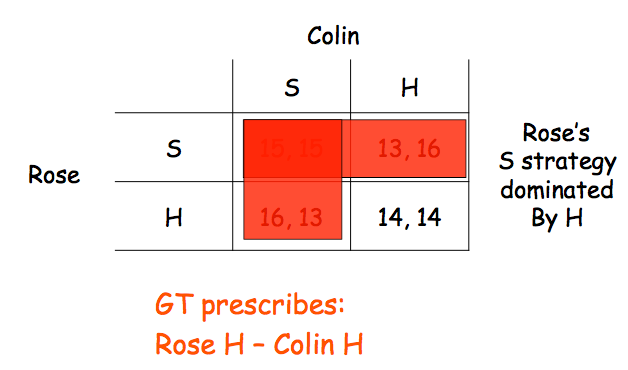
\includegraphics[scale=.35]{images/step2}
\caption{Iteration 2}
\label{figure7}
\end{figure}\\
In this case, we have only one final state but it may happen that we have more than one final state or no final state at all. 
\subsection{Pure Strategy Nash Equilibrium}
Nash equilibrium is a stable state of a system that involves several interacting players in which no player can gain by change of a strategy as long as all other participants remain unchanged. To see what this means, imagine that each player is told the strategies of the others. Suppose then that each player asks themselves: "Knowing the strategies of the other players, and treating the strategies of the other players as set in stone, can I benefit by changing my strategy?"
If any player could answer "Yes", then that set of strategies is not a Nash equilibrium. But if every player prefers not to switch (or is indifferent between switching and not) then the strategy profile is a Nash equilibrium.\\
Example:-
\begin{figure}[h!]
\centering
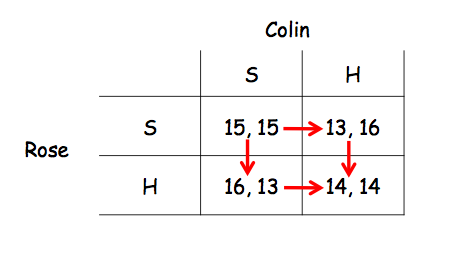
\includegraphics[scale=.35]{images/NE}
\caption{State HH is a Nash Equilibrium.}
\label{figure8}
\end{figure}

In the Figure~\ref{figure8}, the red arrow denotes the movement or the likeness of a particular state by other states. The head of arrow is the state which produces more gain to a player. Ex: If Rose chooses "S" then colin can either choose S or H. We can see in the figure that choosing H gives a gain of 16 whereas choosing S gives a gain of 15. So, we put an arrow from SS to SH. This means that if ever Rose plays S, Colin will play H. Similary, If colin chooses H. Rose will play H. We identify a nash equilibrium by a state which has only incoming edges. Here, state HH is the only state with incoming edges.\\

\subsection{Mixed Strategy Equilibria}

There may exists game where there are no pure strategy nash equilibrium. In that case, we resort to Mixed strategy approach. Fig~\ref{figure9} is an example where no pure strategy nash equilibrium exists.

\begin{figure}[h!]
\centering
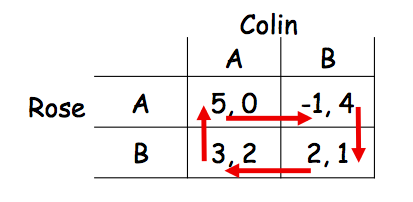
\includegraphics[scale=.35]{images/GamewoNE}
\caption{No Nash equilibrium exists}
\label{figure9}
\end{figure}

Let's us formulate the mixed strategy equilibria of the Fig~\ref{figure9}:-\\
\begin{itemize}
    \item Assign probabilities for Rose's strategies. Say, she has \textbf{p1} probability to choose strategy A and \textbf{(1 - p1)} probability to choose strategy B. 
\begin{figure}[h!]
\centering
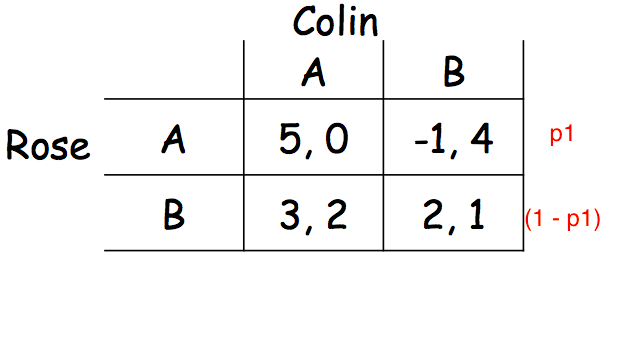
\includegraphics[scale=.35]{images/mix-step1}
\caption{Rose's prob to choose strategy A and B.}
\label{figure10}
\end{figure}
    \item Colin decides to play. He can either play $A$ or $B$. The expected gain for him could be described like in Fig~\ref{figure11}. By solving these two equation we get $p1 = 1/5$. So Rose should choose A with probability $1/5$ and B with probability $4/5$. 
\begin{figure}[h!]
\centering
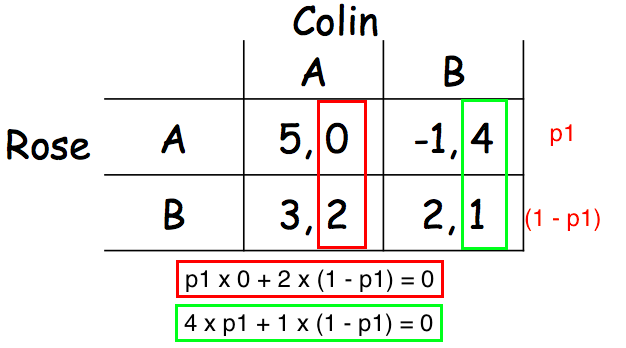
\includegraphics[scale=.35]{images/mix-step2}
\caption{Expected gain for Colin.}
\label{figure11}
\end{figure}
    \item We consider similarly for Colin. With probability q1 to choose strategy A and (1 - q1) to choose B. After writing the expected gain for Rose like in fig~\ref{figure12} We get $q1 = 3/5$.
\begin{figure}[h!]
\centering
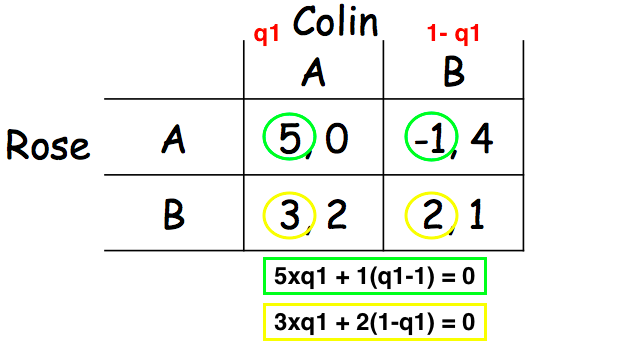
\includegraphics[scale=.35]{images/mix-step3}
\caption{Expected gain for Rose.}
\label{figure12}
\end{figure}
    \item We find that the probability distribution should be (1/5, 4/5) for Rose and (3/5, 2/5) for Colin at equilibrium. Rose gains 13/5 and Colin gains 8/5.
\end{itemize}

\subsection{Auctions}

An auction is a process of buying or selling good by placing bids on it. In game theory, auctions are usually the best method to know the value of a certain good. For ex:- Google doesn't know how much an ad must pay in order to be shown in the search results. So, it holds an auction for the ad spot and the advertisers then starts placing bids to get that spot. Google also takes into account the location, the search query, the brand and other factors when holding the auction but for now we focus only on the auction part.\\

\subsubsection{\textbf{Game Theoretical Model}}\\
\begin{itemize}
    \item There are $N$ players (also called bidders).
    \item Player $i$ places bid $b_i$. $b_i$ are also the strategies of the player $i$.
    \item Player $i$ evaluates the good at value $v_i$.
    \item Player $i$ pays $p_i$ if he gets the good.
    \item Utility of player $i$ is:
    \begin{itemize}
        \item $v_i$ - $p_i$ if player $i$ gets the good.
        \item 0 otherwise.
    \end{itemize}
    \item Values of good $v_i$ are independent and private.
\end{itemize}

\subsubsection{\textbf{Types of Auctions}}
\begin{itemize}
    \item $2^{nd}$ price and ascending bids (English auctions).
    \begin{itemize}
        \item Player with the highest bid gets the good and pays the price equal to the second highest bid. 
        \item A dominant strategy exist in this case which is bid what you really think the value of the good could be. i.e $b_i$ = $v_i$. Why? 
        \begin{itemize}
            \item Case 1: Let $b_i = v_i$ be the highest bid, this means that what you bid is equal to the value then bidding more would still not change the price you must pay is the $2^{nd}$ highest price of the auction. Paying less means you aren't the highest bidder anymore, so you lose the product.
            \item Case 2: Let $b_i$ = $v_i$ not the highest bid, this means if you would had paid more than the highest bidder meaning you lie to yourself and pay more than what you think the worth is. If you would have paid less then it still doesn't make you the highest bidder so it doesn't change anything.
        \end{itemize}
    \end{itemize}
    \item $1^{st}$ price and descending bids (Dutch auctions).
    \begin{itemize}
        \item Auctioneer begins with a high asking price.
        \item The price is lowered until some participant is willing to accept the auctioneer's price, or a predetermined reserve price (the seller's minimum acceptable price) is reached. 
        \item The winning participant pays the last announced price.
        \item Payoff to $i$ is defined as 0 if $b_i$ isn't the winning bid else the payoff is $v_i$ - $b_i$.
        \item Being honest, is not the dominant strategy in this case. By bidding your true value, you would get a payoff of 0 if you lose and you would also get a payoff of 0 if you win, since you’d pay exactly what it was worth to you. As a result, the optimal way to bid in a first-price auction is to “shade” your bid slightly downward, so that if you win you will get a positive payoff. But if you lower this value too much it means that you may not be the highest bid anymore, if you lower it too close to $v_i$ then the payoff is close to $0$.
    \end{itemize}
\end{itemize}

\begin{thebibliography}{alpha}
	
	\bibitem{Kel14} Frank Kelly and Elena Yudovina,
	\newblock Stochastic Networks.
	\newblock {\em Cambridge Press}, 2014.
	
	\bibitem{Giovanni} Giovanni Neglia.
	\newblock Slides: Introduction to Game Theory.
    \newblock  INRIA – EPI Maestro 18 January 2017
    
    \bibitem{Giovanni} Giovanni Neglia.
	\newblock Slides: Auctions.
    \newblock INRIA – EPI Maestro 18 January 2017
	
\end{thebibliography}